\subsection{Alpha Particle X-ray Spectrometer (APXS)}
\initial{T}he APXS is a spectrometer sitting on Curiosity's robot arm.
As its ancestors on the previous rovers the spectrometer is used to identify chemical elements in rock and soil on the Martian surface.
There are some differences, though.
The APXS on Curiosity is better!

\begin{center}
	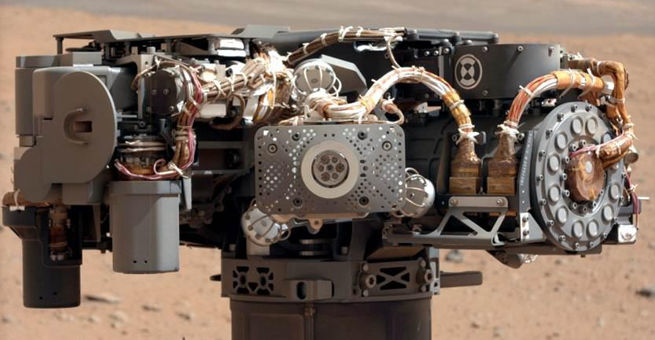
\includegraphics[width=0.45\textwidth]{curiosity_apxs.jpg}
\end{center}

The software controlling Curiosity's arm is an improvement over the previous rovers.
This lets the arm get closer to samples on the ground while keeping the instruments safe.
In addition, the amount of radioactive material used in the source has been doubled, which increases the intensity of the ray.
Since the instruments have to operate at low temperatures, Curiosity's APXS has also been equipped with an electrical solid state cooler which lets it function during the Martian daytime.
Spirit and Opportunity could only use their APXS during night on Mars.

Most of the minerals examined contains elements like sodium, magnesium, aluminum, silicon, calcium, iron and sulfur.
APXS can also detect traces of important elements that take part in different salts: sulfur, chlorine and bromide.
These trace elements can be signs of former interactions with water.

After APXS has studied the samples, Curiosity decides if any other tests should be conducted.
The information from APXS is also used to figure out how the stone formations in the area close to the rover could have formed and changed over time.

The radioactive element curium (Cm$^{244}$) is used as a source for the alpha particles.
The element has a half life of 18.1 years, which suits this kind of long term mission.
Even after more than seven years the decrease in activity will be negligible.

The alpha particles emitted are used to excite atoms in the samples, which responds by emitting X-rays afterwards.
These X-rays will be emitted in all directions and the ones coming back towards Curiosity's robot arm can be used in spectroscopy.

Throughout history the different APXS-instruments on the rovers have given us a lot of important data.
Therefore it was brought yet again on Curiosity, and therefore research is still continuing to improve the technique and refine how we will search for water and traces of it in the future.